\section{设计调研}

\subsection{用户调研}

为了分析自动三维生成技术的用户需求及使用场景，本研究采用半结构化访谈的方法，对三维内容创作者进行了深入调研。访谈旨在了解用户群体特征、使用频率、主要应用场景以及对自动化生成工具的需求与体验。

\subsubsection{调研方法}

本次用户调研主要采用半结构化访谈与问卷结合的方式。访谈对象涵盖：

\begin{itemize}
  \item \textbf{专业用户}：游戏开发人员、影视特效师、三维建模师，共 3 名。
  \item \textbf{非专业用户}：三维内容爱好者、学生及自媒体创作者，共 10 名。
\end{itemize}

访谈内容包括：用户日常三维内容制作流程、对自动生成工具的使用频率、使用中遇到的问题、对材质自动生成和迁移功能的需求，以及对未来工具改进的期望。

每次访谈时长约 30-45 分钟，记录访谈音频并整理访谈笔记。通过对问卷与访谈笔记的定性分析，总结出用户画像与使用特点。

\subsubsection{主要调研发现}

根据访谈结果，可归纳如下特点：

\begin{enumerate}
  \item \textbf{用户群体庞大且多样}：  
  大多数用户表示在日常工作或学习中频繁使用三维建模工具。访谈显示，非专业用户对自动化材质生成功能依赖度更高，专业用户则关注生成效果的可控性与风格一致性。

  \item \textbf{使用场景广泛}：  
  用户将自动三维生成技术应用于多个场景，包括游戏关卡设计、虚拟场景搭建、影视特效制作、在线内容创作及教育培训。访谈中大多数用户表示在实际工作中希望能快速生成统一风格的材质，以节省人工绘制纹理的时间。

  \item \textbf{核心需求集中}：  
  通过访谈整理发现，用户对自动三维生成工具的核心需求集中在：
  \begin{itemize}
    \item 快速生成符合模型结构的材质贴图；
    \item 能够将参考模型的风格迁移到目标白模；
    \item 提供可视化预览工具以快速评估生成结果；
    \item 简单易用的 Web 平台，降低安装和学习成本。
  \end{itemize}

  \item \textbf{用户痛点}：  
  用户普遍反馈，目前工具在材质生成一致性、复杂纹理处理以及跨模型迁移效果上存在局限，尤其是材质迁移部分仍需大量人工干预。
\end{enumerate}

\subsubsection{用户旅程图分析}

基于访谈结果，本研究构建了用户在使用自动三维生成工具过程中的旅程图（图\ref{fig:user_journey}）。
\begin{figure}[htbp]
    \centering
    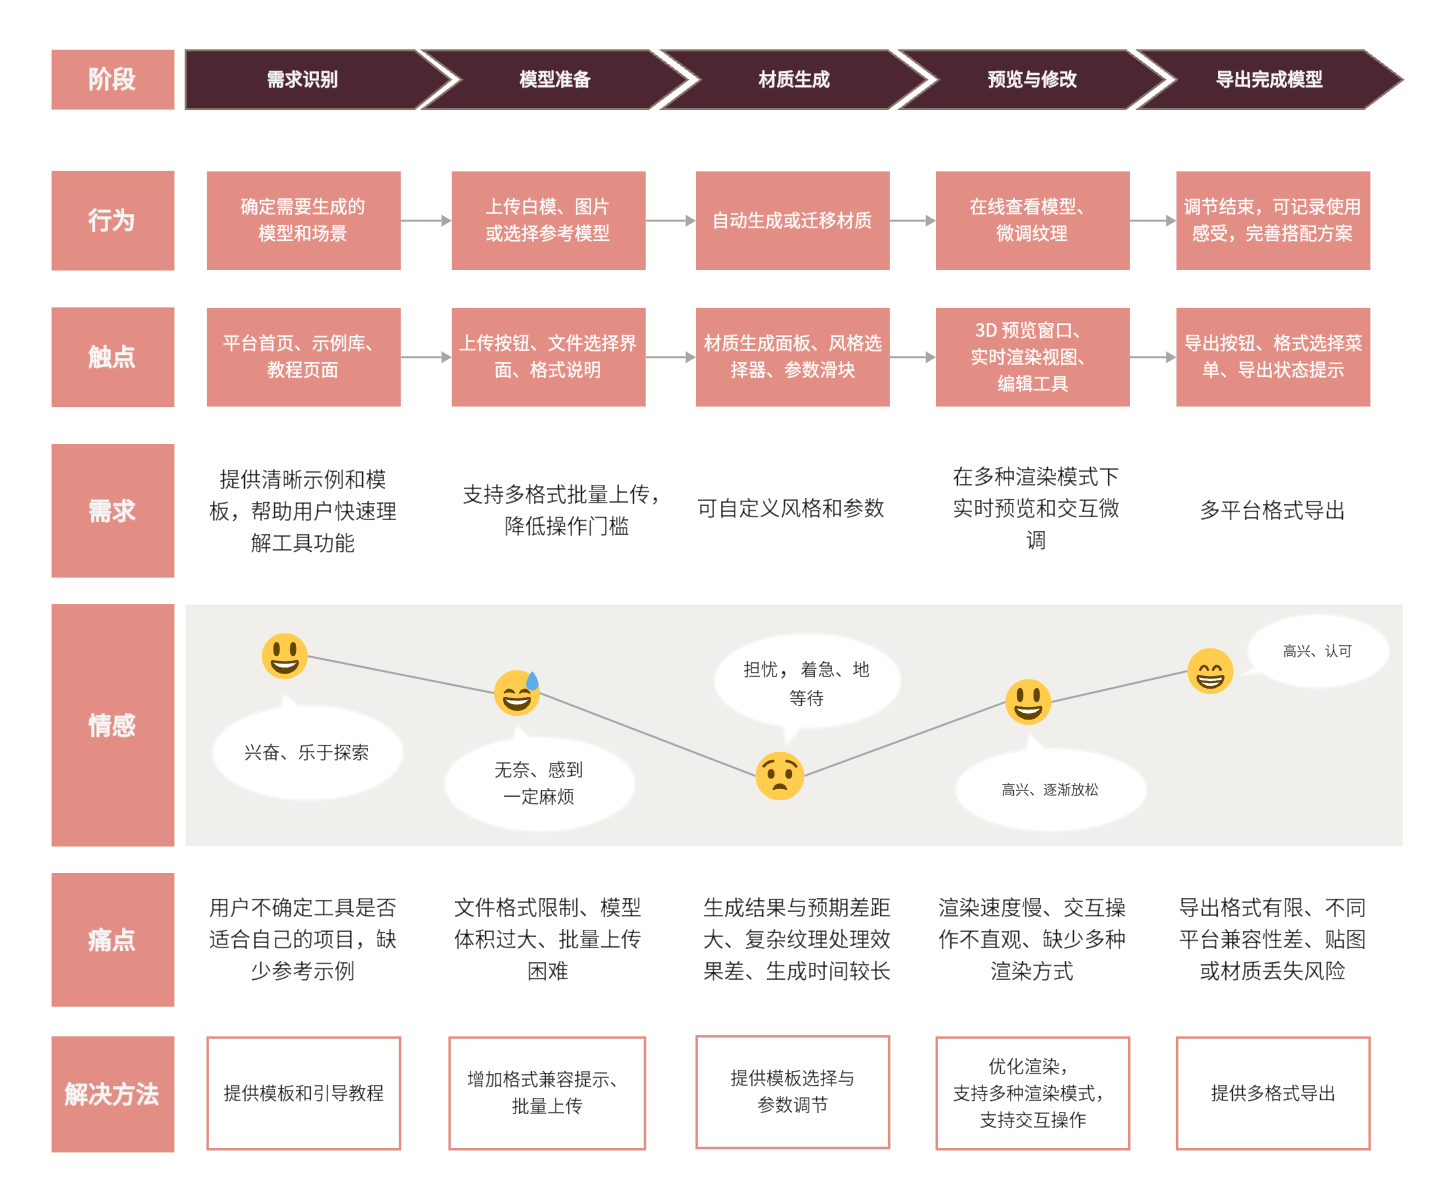
\includegraphics[width=0.8\textwidth]{figure/proposal/journey.png}
    \caption{面向 Web 三维生成系统的用户旅程图}
    \label{fig:user_journey}
\end{figure}
用户旅程分为五个阶段：需求识别、模型准备、材质生成、预览与修改及导出与应用。  

旅程图清晰展示了用户在各阶段的操作、体验情绪、痛点以及对工具的需求。例如，在材质生成阶段，用户普遍对生成效果不够精细和风格不统一感到沮丧，这直接体现了系统在材质迁移与风格控制方面的改进空间。  

通过旅程图分析，可以为系统功能设计提供指导，包括增强风格自定义、提供实时预览、优化导出兼容性等，从而提升整体用户体验。

\subsubsection{小结}

通过访谈调研，本研究明确了目标用户群体、使用习惯以及对自动三维生成和材质迁移功能的核心需求。这为系统的功能设计、交互流程以及算法优化提供了直接依据，同时也为后续的 Web 平台开发提供了用户体验参考。

\subsection{基于 Web 的三维材质生成平台调研}

为了明确当前在线三维生成工具在功能实现、用户体验与交互设计上的特点，  
本节对典型的 Web 平台进行了调研分析。  
所选平台包括国内外较为代表性的混元3D、Tripo 以及 SAM 3D，  
以便从不同设计理念、实现路径和用户交互方式上进行比较研究。  

\subsubsection{腾讯混元3D 平台分析}

混元3D 是腾讯公司推出的一款基于 AI 技术的在线三维生成平台，  
支持用户通过文本描述或图像草稿快速生成 3D 模型。  
该平台以其简单易用、快速生成、高度可定制化等特点，  
受到了广大用户的欢迎。  

\paragraph{逻辑设计}  
混元3D 的整体逻辑设计遵循“三步生成流程”：输入—配置参数—生成与预览。  
用户首先选择输入类型（如文本、图像或草图），  
然后配置输出细节程度（如面数、PBR 材质启用）等参数，  
最后触发云端 AI 生成并在浏览器中预览结果。  
该逻辑设计旨在将复杂的三维生成任务抽象为用户可理解的操作步骤，  
从而降低场景使用门槛。  

\paragraph{界面与美术设计}  
混元3D 的界面布局以简洁直观为主，  
页面左侧为输入选项卡，中心区域为模型预览和展示区，右侧则是渲染调节区。  
整体视觉风格采用深黑色背景，与之对比鲜明的按钮提示用户操作步骤，  
能够引导用户逐步完成生成流程。  
其美术设计注重控制视图清晰度，  
避免复杂 UI 元素分散用户注意力，  
符合在线快速生成功能的定位。  

\paragraph{交互设计}  
交互层面，混元3D 支持多输入方式切换，  
用户可以无缝地从文本描述切换到图像上传或草图输入，  
同时配置参数的实时反馈（如模型选择和面数调节）  
使得用户在生成前对输出有初步控制。  
生成后内嵌 3D 预览器支持旋转、缩放等基础交互，  
使用户可直观评估结果。  

\subsubsection{Tripo 平台分析}

Tripo 是一款面向在线 AI 3D 模型生成和编辑的综合平台，  
支持从文本、图片等多种输入快速生成 3D 模型，  
并提供智能分割、自动贴图以及自动绑定等功能。  

\paragraph{逻辑设计}  
Tripo 的设计逻辑强调“一体化 3D 生成工作流”。  
基础生成流程包括上传图像或文本输入 → 模型生成 → 模型编辑（如分割、重拓扑） → 导出与应用。  
平台还融入了智能分割模块，  
用于将复杂模型自动拆分为可编辑部件，  
并支持自动 Rigging（骨骼绑定）等后处理步骤，  
从几何生成扩展到可用性强化。  

\paragraph{界面与美术设计}  
Tripo 的界面设计偏向“创意工作空间”，  
将生成控制面板、模型预览区域、工具栏功能区分在不同面板上，  
使专业用户可以快速定位所需功能。  
配色采用深黑色背景和高对比操作组件，  
视觉上兼顾信息密度和可读性。   

\paragraph{交互设计}  
Tripo 在交互方面提供了较丰富的模型编辑能力。  
生成后的模型可以单击选择不同部件，  
用户可对局部几何或纹理做调整，  
并能通过可视化工具即时查看修改效果。  
此外平台支持模型自动 Rigging、T‑Pose 导出等功能，  
使得生成结果更易于在游戏和动画管线中应用。  

\subsubsection{SAM 3D 平台分析}

SAM 3D 是基于 Meta 研究的 3D 重建与生成技术的在线实现，  
针对从单一图片生成带有几何和纹理的 3D 对象或场景。  
该平台具有先进的语义分割与推理能力，  
能通过单张图像推断出完整三维结构。  
与其他平台不同的是，SAM 3D 支持用户在生成前编辑输入图片的背景，  
这使得用户可以更灵活地控制模型生成环境和场景效果。  

\paragraph{逻辑设计}  
SAM 3D 的逻辑设计聚焦于“单视图 3D 重建流程”。  
这一流程通常从用户上传图像开始，  
用户可在上传阶段修改图片背景以优化生成效果，  
然后通过内置的高级分割算法识别图像中的目标对象，  
再在云端 AI 模型中推断完整几何结构和相应纹理，  
最终将 3D 模型导出为标准格式。  

\paragraph{界面与美术设计}  
SAM 3D 界面采用极简风格：  
左侧为图像上传与背景编辑区，  
上传或修改后显示实时处理状态，  
并在结果生成后切换至 3D 预览界面。  
整体界面功能清晰、元素简洁，  
重点突出输入、背景调整与输出的核心交互步骤。  

\paragraph{交互设计}  
在交互体验上，SAM 3D 提供拖拽上传、图片背景编辑、自动对象检测与选择等便捷方式。  
用户可以在上传阶段自由调整图像背景，  
生成结果的 3D 预览支持基本视角操作，  
并可导出多种格式，  
以便在三维引擎中进一步使用。

\subsubsection{综合比较与启示}

通过对上述三种平台的调研可以看出，  
目前基于 Web 的三维生成平台在逻辑设计上均强调“简单输入 → 可控参数 → 实时生成”的流程；  
界面方面多采用简洁清晰的布局，使用户易于理解操作流程；  
交互设计则兼顾基础预览与部分编辑功能，  
从生成、预览、调整到导出尽量减少用户负担。  
这些设计理念对本研究中 Web 平台的功能划分、界面布局与交互流程设计都有重要参考价值。

\section{算法调研}


